%%%%%%%%%%%%%%%%%%%%%%%%%%%%%%%%%%%%%%%%%%%%%%%%%%%%%%%%%%%%%%%
%% OXFORD THESIS TEMPLATE

% Use this template to produce a standard thesis that meets the Oxford University requirements for DPhil submission
%
% Originally by Keith A. Gillow (gillow@maths.ox.ac.uk), 1997
% Modified by Sam Evans (sam@samuelevansresearch.org), 2007
% Modified by John McManigle (john@oxfordechoes.com), 2015
%
% This version Copyright (c) 2015-2023 John McManigle
%
% Broad permissions are granted to use, modify, and distribute this software
% as specified in the MIT License included in this distribution's LICENSE file.
%

% I've (John) tried to comment this file extensively, so read through it to see how to use the various options.  Remember
% that in LaTeX, any line starting with a % is NOT executed.  Several places below, you have a choice of which line to use
% out of multiple options (eg draft vs final, for PDF vs for binding, etc.)  When you pick one, add a % to the beginning of
% the lines you don't want.


%%%%% CHOOSE PAGE LAYOUT
% The most common choices should be below.  You can also do other things, like replacing "a4paper" with "letterpaper", etc.

% This one will format for two-sided binding (ie left and right pages have mirror margins; blank pages inserted where needed):
%\documentclass[a4paper,twoside]{ociamthesis}
% This one will format for one-sided binding (ie left margin > right margin; no extra blank pages):
%\documentclass[a4paper]{ociamthesis}
% This one will format for PDF output (ie equal margins, no extra blank pages):
\documentclass[a4paper,nobind]{ociamthesis} 



%%%%% SELECT YOUR DRAFT OPTIONS
% Three options going on here; use in any combination.  But remember to turn the first two off before
% generating a PDF to send to the printer!

% This adds a "DRAFT" footer to every normal page.  (The first page of each chapter is not a "normal" page.)
%\fancyfoot[C]{\emph{DRAFT Printed on \today}}  

% This highlights (in blue) corrections marked with (for words) \mccorrect{blah} or (for whole
% paragraphs) \begin{mccorrection} . . . \end{mccorrection}.  This can be useful for sending a PDF of
% your corrected thesis to your examiners for review.  Turn it off, and the blue disappears.
%\correctionstrue


%%%%% BIBLIOGRAPHY SETUP
% Note that your bibliography will require some tweaking depending on your department, preferred format, etc.
% The options included below are just very basic "sciencey" and "humanitiesey" options to get started.
% If you've not used LaTeX before, I recommend reading a little about biblatex/biber and getting started with it.
% If you're already a LaTeX pro and are used to natbib or something, modify as necessary.
% Either way, you'll have to choose and configure an appropriate bibliography format...

% The science-type option: numerical in-text citation with references in order of appearance.
\usepackage[style=numeric-comp, sorting=none, backend=biber, doi=false, isbn=false]{biblatex}
\newcommand*{\bibtitle}{References}

% The humanities-type option: author-year in-text citation with an alphabetical works cited.
%\usepackage[style=authoryear, sorting=nyt, backend=biber, maxcitenames=2, useprefix, doi=false, isbn=false]{biblatex}
%\newcommand*{\bibtitle}{Works Cited}

% This makes the bibliography left-aligned (not 'justified') and slightly smaller font.
\renewcommand*{\bibfont}{\raggedright\small}

% Change this to the name of your .bib file (usually exported from a citation manager like Zotero or EndNote).
\addbibresource{references.bib}


% Uncomment this if you want equation numbers per section (2.3.12), instead of per chapter (2.18):
%\numberwithin{equation}{subsection}



%%%%% THESIS / TITLE PAGE INFORMATION
% Everybody needs to complete the following:
\title{Neutrinos!ND up!}
\author{Weijun Li}
\college{The Queen's College}

% Master's candidates who require the alternate title page (with candidate number and word count)
% must also un-comment and complete the following three lines:
%\masterssubmissiontrue
%\candidateno{933516}
%\wordcount{28,815}

% Uncomment the following line if your degree also includes exams (eg most masters):
%\renewcommand{\submittedtext}{Submitted in partial completion of the}
% Your full degree name.  (But remember that DPhils aren't "in" anything.  They're just DPhils.)
\degree{Doctor of Philosophy}
% Term and year of submission, or date if your board requires (eg most masters)
\degreedate{Michaelmas 2025}


%%%%% YOUR OWN PERSONAL MACROS
% This is a good place to dump your own LaTeX macros as they come up.

% To make text superscripts shortcuts
	\renewcommand{\th}{\textsuperscript{th}} % ex: I won 4\th place
	\newcommand{\nd}{\textsuperscript{nd}}
	\renewcommand{\st}{\textsuperscript{st}}
	\newcommand{\rd}{\textsuperscript{rd}}

%%%%% THE ACTUAL DOCUMENT STARTS HERE
\begin{document}



%%%%% CHOOSE YOUR LINE SPACING HERE
% This is the official option.  Use it for your submission copy and library copy:
\setlength{\textbaselineskip}{22pt plus2pt}
% This is closer spacing (about 1.5-spaced) that you might prefer for your personal copies:
%\setlength{\textbaselineskip}{18pt plus2pt minus1pt}

% You can set the spacing here for the roman-numbered pages (acknowledgements, table of contents, etc.)
\setlength{\frontmatterbaselineskip}{17pt plus1pt minus1pt}

% Leave this line alone; it gets things started for the real document.
\setlength{\baselineskip}{\textbaselineskip}


%%%%% CHOOSE YOUR SECTION NUMBERING DEPTH HERE
% You have two choices.  First, how far down are sections numbered?  (Below that, they're named but
% don't get numbers.)  Second, what level of section appears in the table of contents?  These don't have
% to match: you can have numbered sections that don't show up in the ToC, or unnumbered sections that
% do.  Throughout, 0 = chapter; 1 = section; 2 = subsection; 3 = subsubsection, 4 = paragraph...

% The level that gets a number:
\setcounter{secnumdepth}{2}
% The level that shows up in the ToC:
\setcounter{tocdepth}{2}


%%%%% ABSTRACT SEPARATE
% This is used to create the separate, one-page abstract that you are required to hand into the Exam
% Schools.  You can comment it out to generate a PDF for printing or whatnot.
\begin{abstractseparate}
	Your abstract text goes here.  Check your departmental regulations, but generally this should be less than 300 words.  See the beginning of Chapter~\ref{ch:2-litreview} for more.

Worked on upgrade, new physics potential

Did a few analyses based on the upgrade:
    - ESC
    - TL pi
    - COM
    - TKI

However, not enough time to look at data, hence did a tuning project and a sens extraction. % Create an abstract.tex file in the 'text' folder for your abstract.
\end{abstractseparate}


% JEM: Pages are roman numbered from here, though page numbers are invisible until ToC.  This is in
% keeping with most typesetting conventions.
\begin{romanpages}

% JEM: By default, this template uses the traditional Oxford "Belt Crest". Un-comment the following
% line to use the newer, "Blue Square" logo:
% \renewcommand{\crest}{{\includegraphics[width=4.2cm, height=4.2cm]{figures/newlogo.pdf}}}

% Title page is created here
\maketitle

%%%%% DEDICATION -- If you'd like one, un-comment the following.
%\begin{dedication}
%This thesis is dedicated to\\
%someone\\
%for some special reason\\
%\end{dedication}

%%%%% ACKNOWLEDGEMENTS -- Nothing to do here except comment out if you don't want it.
\begin{acknowledgements}
 	\subsection*{Personal}

Thank you!!!!!

% \subsection*{Institutional}

% If you want to separate out your thanks for funding and institutional support, I don't think there's any rule against it.  Of course, you could also just remove the subsections and do one big traditional acknowledgement section.

% Lorem ipsum dolor sit amet, consectetur adipiscing elit. Ut luctus tempor ex at pretium. Sed varius, mauris at dapibus lobortis, elit purus tempor neque, facilisis sollicitudin felis nunc a urna. Morbi mattis ante non augue blandit pulvinar. Quisque nec euismod mauris. Nulla et tellus eu nibh auctor malesuada quis imperdiet quam. Sed eget tincidunt velit. Cras molestie sem ipsum, at faucibus quam mattis vel. Quisque vel placerat orci, id tempor urna. Vivamus mollis, neque in aliquam consequat, dui sem volutpat lorem, sit amet tempor ipsum felis eget ante. Integer lacinia nulla vitae felis vulputate, at tincidunt ligula maximus. Aenean venenatis dolor ante, euismod ultrices nibh mollis ac. Ut malesuada aliquam urna, ac interdum magna malesuada posuere.
\end{acknowledgements}

%%%%% ABSTRACT -- Nothing to do here except comment out if you don't want it.
\begin{abstract}
	Your abstract text goes here.  Check your departmental regulations, but generally this should be less than 300 words.  See the beginning of Chapter~\ref{ch:2-litreview} for more.

Worked on upgrade, new physics potential

Did a few analyses based on the upgrade:
    - ESC
    - TL pi
    - COM
    - TKI

However, not enough time to look at data, hence did a tuning project and a sens extraction.
\end{abstract}

%%%%% MINI TABLES
% This lays the groundwork for per-chapter, mini tables of contents.  Comment the following line
% (and remove \minitoc from the chapter files) if you don't want this.  Un-comment either of the
% next two lines if you want a per-chapter list of figures or tables.
\dominitoc % include a mini table of contents
%\dominilof  % include a mini list of figures
%\dominilot  % include a mini list of tables

% This aligns the bottom of the text of each page.  It generally makes things look better.
\flushbottom

% This is where the whole-document ToC appears:
\tableofcontents

\listoffigures
	\mtcaddchapter
% \mtcaddchapter is needed when adding a non-chapter (but chapter-like) entity to avoid confusing minitoc

% Uncomment to generate a list of tables:
%\listoftables
%	\mtcaddchapter

%%%%% LIST OF ABBREVIATIONS
% This example includes a list of abbreviations.  Look at text/abbreviations.tex to see how that file is
% formatted.  The template can handle any kind of list though, so this might be a good place for a
% glossary, etc.
% First parameter can be changed eg to "Glossary" or something.
% Second parameter is the max length of bold terms.
\begin{mclistof}{List of Abbreviations}{3.2cm}

\item[1-D, 2-D] One- or two-dimensional, referring in this thesis to spatial dimensions in an image.

\item[TKI] Transverse Kinematic Imbalance
\item[COM] Centre-of-momentum

\end{mclistof} 


% The Roman pages, like the Roman Empire, must come to its inevitable close.
\end{romanpages}


%%%%% CHAPTERS
% Add or remove any chapters you'd like here, by file name (excluding '.tex'):
\flushbottom
\begin{savequote}[8cm]
\textlatin{Neque porro quisquam est qui dolorem ipsum quia dolor sit amet, consectetur, adipisci velit...}

There is no one who loves pain itself, who seeks after it and wants to have it, simply because it is pain...
  \qauthor{--- Cicero's \textit{de Finibus Bonorum et Malorum}}
\end{savequote}

\chapter{\label{ch:1-intro}Introduction} 

\minitoc

\section{Motivation}
   One of the big mysteries of modern physics is the matter-antimatter asymmetry observed in our universe. A key ingredient to a possible answer to this asymmetry is the charge-parity (CP) violation. However, the CP violation in weak interaction of the quark sector is measured to be insufficient for the observed matter-antimatter asymmetry and the CP violation in strong interaction of the quarks is surprisingly infinitesimal, which is considered by many a puzzle on its own - the Strong CP Problem. Hence, the only remaining source of CP violation in the Standard Model (SM) of particle physics lies in the weak interaction of leptons, which is quantified by a complex phase, $\dcp$, in the lepton mixing matrix, the Pontecorvo–Maki–Nakagawa–Sakata (PMNS) matrix. If CP is violated in leptons, i.e. $\sin{\dcp}\neq0$ neutrino and anti-neutrino would oscillate differently, allowing the possibility of asymmetric production of matter and anti-matter. Hence, a precise measurement of $\dcp$ would be a big step toward solving this problem. 
   
   More specifically, $\dcp$ can be measured in long-baseline neutrino experiments, for example, the Tokai-to-Kamioka (T2K) experiment\cite{T2KEXP}. T2K is a long-baseline neutrino experiment located in Japan. The neutrino source is generated in J-PARC in Tokai. A near detector, ND280, is placed at $280\textrm{m}$ from the generation point, and a far detector, the Super Kamiokande (SK), is situated 296km away. As neutrinos interact extremely weakly, direct measurement is not yet possible. These detectors measure the neutrino energy spectra from the product particles from the interaction between neutrinos and hydrocarbons in ND280 and water molecules in SK. The difference between neutrino oscillation and anti-neutrino oscillation can be measured by comparing the neutrino energy spectra observed at the far and near detectors in the neutrino mode and the anti-neutrino mode. In 2020, the Tokai-to-Kamioka (T2K) experiment\cite{T2KEXP} has made the first measurement of $\dcp$\cite{T2Knature}, which ruled out CP conservation at the $95\%$ confidence level. It is an impressive first step, but it is still limited both by statistical and systematic uncertainties. 

   SK will be replaced by Hyper-Kamiokande (Hyper-K) in 2027, which is much larger than SK and would increase statistics many-fold. 
   The uncertainties in the measurement of $\dcp$ will be systematics dominant. One of the most significant systematic uncertainties lies in the neutrino-nucleus interaction modelling. Although the neutrino source beam energy spectrum is well studied, the energy reconstruction of each neutrino is not directly measurable as it leaves no visible track in detectors. Thus, we have to rely on approximate neutrino-nucleus interaction models to reconstruct its energy from the interaction products, of which the hadrons and leptons could be detected and their energy could be measured if energetic enough. Hence, reducing particle energy measurement uncertainty and developing a more sophisticated neutrino-nucleus interaction model is crucial for the future $\dcp$ measurement. The ND280 has been upgraded to achieve this goal and the research of my thesis centres around this upgrade. 

   This report is structured as follows: Sec.~\ref{sec:ndup} briefly describes the hardware upgrade. 
   The improvement on physical measurements are investigated based on Monte Carlo (MC) simulation, and the results for single particle kinematics and derived observables, such as the Transverse Kinematic Imbalance (TKI) Variables, are presented in Sec.~\ref{sec:spk} and Sec.~\ref{sec:derobs}. 
   The following section, Sec.~\ref{sec:app}, showcases how these improvements could benefit physical analyses. Lastly, Sec.~\ref{sec:summary} summarises the states of my analyses and proposes a plan for the required work. A draft thesis plan is also included in the appendix.
\section{\label{sec:ndup} ND280 Upgrade}
   In the upgrade, the $\piz$ detector is replaced by a suite of sophisticated new sub-detectors, namely the Time-of-flight detector (TOF), two high angle TPCs and the Super Fine Grained Detector (SFGD). 
   The TOF consists of 6 planes of scintillation bars, providing excellent sub-nano second timing resolution. 
   It can effectively veto trespassing particles, thus improving the sample purity.
   The high angle TPCs (HAT) have a new field cage design and new Micromegas, leading to a larger tracking volume and better resolution than the existing vertical TPCs in ND280. 
   The SFGD is the new active target, consisting of about 2 million scintillation cubes, each with a size of $1~\textrm{cm}^3$. 
   The granularity of SFGD improves the high-angle acceptance significantly and thus leads to better phase space matching between the ND and the FD. 
   Moreover, the tracking capabilities are also enhanced by the more precise measurement of energy deposited along the particle track. 
   Hence, detection thresholds are lowered and resolution improved, opening up avenues for novel reconstruction techniques, such as trackless pion reconstruction, and creative construction of variables, like COM variables. 
   The upgrade has finished in April 2024 and the upgraded detector has started taking data in June 2024. An example event display is shown in Fig.~\ref{fig:ndup-evedis}. 

    \begin{figure}[!htb]
        \centering
        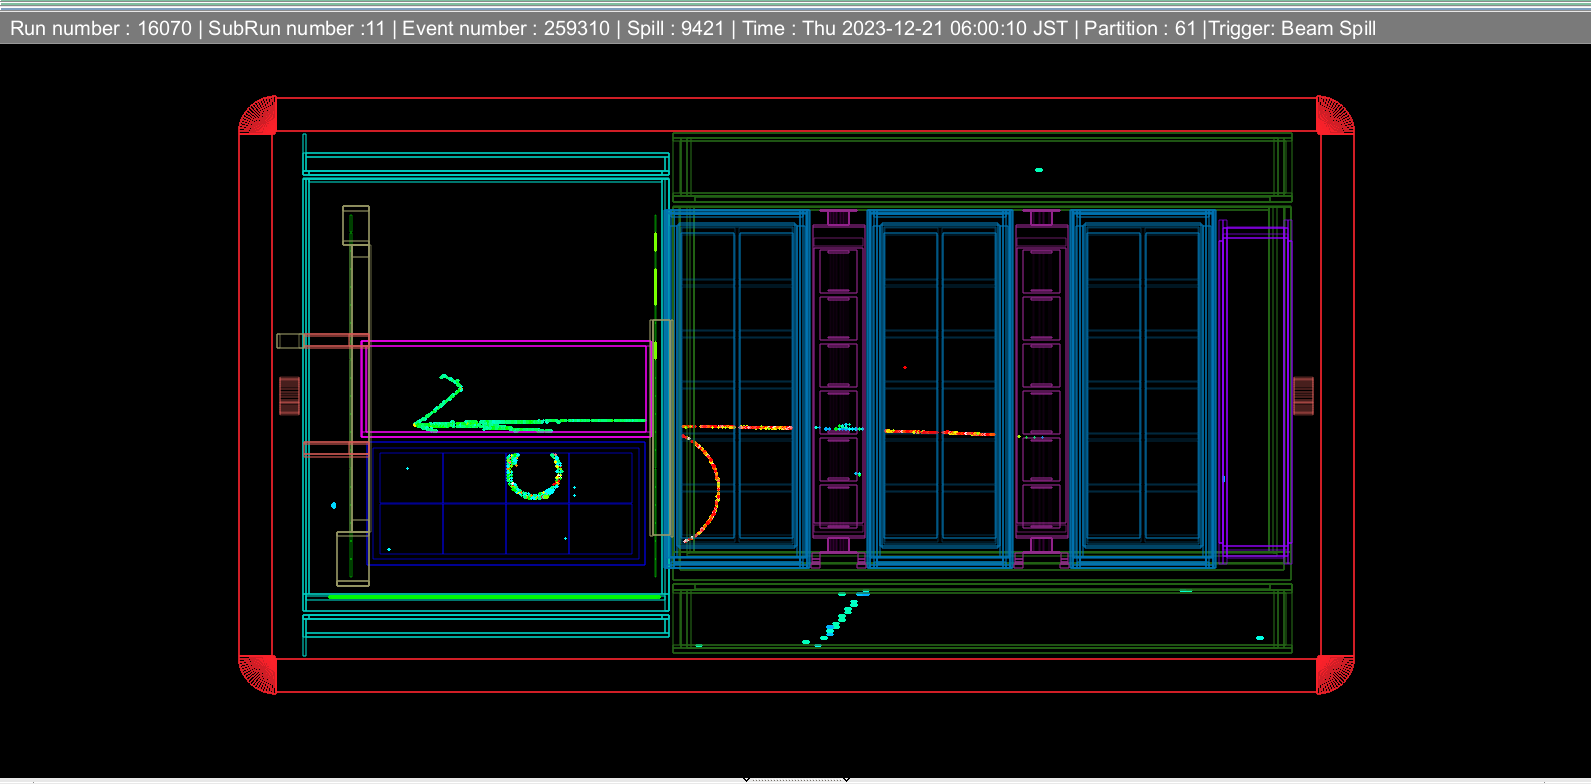
\includegraphics[width=0.5\linewidth]{fig/upgradeEvtDis.png}
        \caption{Event display of a possible $\pi^+$ event.}
        \label{fig:ndup-evedis}
    \end{figure}
\begin{savequote}[8cm]
Alles Gescheite ist schon gedacht worden.\\
Man muss nur versuchen, es noch einmal zu denken.

All intelligent thoughts have already been thought;\\
what is necessary is only to try to think them again.
  \qauthor{--- Johann Wolfgang von Goethe \cite{von_goethe_wilhelm_1829}}

Dancing is more important. --- Pauli
\end{savequote}

\chapter{\label{ch:2-neutrinos}The Field of Neutrinos}

\minitoc

\section{The Past}
\section{The Present}
\section{The Plans}


This document introduction won't serve as a complete primer on \LaTeX.  There are plenty of those online, and googling your questions will often get you answers, especially from \url{http://tex.stackexchange.com}.

Instead, let's talk a little about a few of the features and packages lumped into this template situation.  The \verb|savequote| environment at the beginning of chapters can add some wittiness to your thesis.  If you don't like the quotes, just remove that block.

For when it comes time to do corrections, there are two useful commands here.  First, the \verb|mccorrect| command allows you to highlight a short correction \mccorrect{like this one}.  When the thesis is typeset normally, the correction will just appear as part of the text.  However, when you declare \verb|\correctionstrue| in the main \verb|Oxford_Thesis.tex| file, that correction will be highlighted in blue.  That might be useful for submitting a post-viva, corrected copy to your examiners so they can quickly verify you've completed the task.

\begin{mccorrection}
For larger chunks, like this paragraph or indeed entire figures, you can use the \verb|mccorrection| environment.  This environment highlights paragraph-sized and larger blocks with the same blue colour.
\end{mccorrection}

Read through the \verb|Oxford_Thesis.tex| file to see the various options for one- and two-sided printing, including or excluding the separate abstract page, and turning corrections and draft footer on or off, and the separate option to centre your text on the page (for PDF submission) or offset it (for binding).  There is also a separate option for master's degree submissions, which changes identifying information to candidate number and includes a word count.  (Unfortunately, \LaTeX has a hard time doing word counts automatically, so you'll have to enter the count manually if you require this.)

\section{Cardiac Imaging}\label{app:imaging}

Within months of Röntgen's discovery of the X-ray in \mccorrect{1895}\cite{gagliardi_rontgen_1996}, cardiac pathology was being investigated via non-invasive imaging \cite{gagliardi_cardiac_1996}.  Over the intervening years, cardiac imaging modalities and techniques have advanced significantly.  Clinically, cardiac imaging is used for two broad purposes: diagnosis of pathophysiology and guidance of interventional procedures.  These applications impose different requirements on imaging equipment, image acquisition time, computational complexity, spatial and temporal resolution, and tissue discrimination.  The common diagnostic and interventional cardiac imaging techniques in current clinical practice are reviewed below.  An accessible introduction to the physics of medical imaging can be found in Webb's \textit{Introduction to Biomedical Imaging} \cite{webb_introduction_2002}.  A comprehensive overview of the use of imaging in clinical cardiology is presented in Leeson's \textit{Cardiovascular Imaging} \cite{leeson_cardiovascular_2011}.

\subsection{Diagnostic Imaging}
\label{sub:diagnostic}

Beyond the chest X-ray (`plain film'), the key non-invasive imaging modalities in diagnostic cardiology are echocardiography, magnetic resonance imaging, and X-ray computed tomography, which are reviewed below.  Nuclear medicine, including positron emission tomography (PET) and single-photon emission computed tomography (SPECT), are not discussed here, as they do not play a role in the chapters to follow.

\subsubsection{Echocardiography}

\begin{figure}
\centering\includegraphics[width=0.7\textwidth]{figures/sample/Gray498.png} 
\caption[Four-chamber illustration of the human heart.]{Four-chamber illustration of the human heart.  Clockwise from upper-left: right atrium, left atrium, left ventricle, right ventricle.}
\label{fig:fourchamber}\end{figure}

The use of acoustic waves for medical diagnosis, inspired by naval sonar, was initially developed in the 1940s \cite{gagliardi_ultrasonography_1996}.  By 1954, the first clinically useful cardiac ultrasound -- examining motion of the mitral valve in stenosis -- was reported \cite{edler_ultrasonic_1957}.  These early scans were one-dimensional images (`A-mode'), sometimes repeated to generate a time axis (`M-mode').   The sector-scanning probe was developed in the 1970s \cite{bom_ultrasonic_1971,griffith_sector_1974}, leading to the `B-mode' that a modern cardiologist would recognise as an echocardiogram.



%% APPENDICES %% 
% Starts lettered appendices, adds a heading in table of contents, and adds a
%    page that just says "Appendices" to signal the end of your main text.
\startappendices
% Add or remove any appendices you'd like here:
\begin{savequote}[8cm]
\textlatin{Cor animalium, fundamentum e\longs t vitæ, princeps omnium, Microco\longs mi Sol, a quo omnis vegetatio dependet, vigor omnis \& robur emanat.}

The heart of animals is the foundation of their life, the sovereign of everything within them, the sun of their microcosm, that upon which all growth depends, from which all power proceeds.
  \qauthor{--- William Harvey \cite{harvey_exercitatio_1628}}
\end{savequote}

\chapter{\label{app:1-cardiophys}Review of Cardiac Physiology and Electrophysiology}

\minitoc

\section{HNL Input Parameter Calculations}
\label{sec:hnl-input}
    \subsection{Coordinates transformation between different frames}

    \begin{enumerate}
        \item $M_{N}$, mass of the HNL
        \item $\uae$ and $\uam$, the mixing coffeicient of the extended PMNS matrix between the HNL and the electron neutrino and muon neutrino respectively.
        \item XXXX, position of the centre of the detector relative to the centre of the target (?)
        \item XXXX, angle between the beam axis and the longitudinal axis of the detector.
        \item POT parent scaling, the average number of hadrons produced per POT.
    \end{enumerate}
    As the hadrons produced by the T2K beam are predominantly pions and kaons, the $M_{N}$ range that can be explored from hadron decay is between $140\mev$ to $390\mev$. 
    Furthermore, as the decay channel investigated in this work are the two-body decay channels, namely $\pi$+$e$ and $\pi$+$\mu$, the chosen range for $M_{N}$ is from $140\mev$ (250 if mupi only) to $390\mev$ (???).
    
    $\uae$ and $\uam$ are chosen to be equal to $10^{-7}$. They are chosen to be small such that the first order approximation of the proportionality between the number of observed events and the fourth power of the mixing elements are valid.

    In order to specify the relations bewteen the target position, the beam direction and the detector position accurately, three coordiante systems are used.
    The NEAR frame has the origin inside the target with its $y$ axis parallel to the floor of the target hall.
    The NEAR frame is also the frame used by the NEUT generator.
    The BEAM frame is typically rotated from the NEAR frame with the $z$ axis parallel to the beam direction. 
    The USER frame is the coordiante system setup at ND280 for event selection and analysis.

    Taken from official document, the centre of the USER frame is at $(-3.222,-8.146,280.1)$ in the NEAR frame. 
    The BEAM frame is rotated from the NEAR frame downwards around the $x$-axis by $63.44\mrad$. 
    (CHECK how is 63.44 calculated)

    As \code{BeamHNL} aims to be a cross-experiment package, it requires a standardised flux input, the \code{dk2nu} format. 
    The \code{dk2nu} file is a simple flattree root file that needs to contain the minimally sufficient information for \code{BeamHNL} to work.
    As the T2K flux is available in its specific format, a conversion is required. 
    The required \code{dk2nu} variables and the corresponding variables in a T2K flux file is given in Table~\ref{tab:dk2nu-t2k-conv}.
        

\section{Anatomy}
\label{sec:anatomy}


\section{Cellular Electromechanical Coupling}
\label{sec:electromech}



%%%%% REFERENCES

% JEM: Quote for the top of references (just like a chapter quote if you're using them).  Comment to skip.
\begin{savequote}[8cm]
The first kind of intellectual and artistic personality belongs to the hedgehogs, the second to the foxes \dots
  \qauthor{--- Sir Isaiah Berlin \cite{berlin_hedgehog_2013}}
If I see further, that is because I am on the shoulders of giants.
    \qauthor{--- Sir Issac Newton}
\end{savequote}

\setlength{\baselineskip}{0pt} % JEM: Single-space References

{\renewcommand*\MakeUppercase[1]{#1}%
\printbibliography[heading=bibintoc,title={\bibtitle}]}


\end{document}
